\documentclass{article}
\usepackage[UTF8]{ctex}
\usepackage{amsmath,mathtools,geometry,pgfplots,float,mathrsfs,caption}
\pgfplotsset{compat=1.15}
\usetikzlibrary{arrows}
\usetikzlibrary[patterns]
\geometry{scale=0.7}

\title{第四题整理}
\author{ }
\date{ }

\begin{document}
\maketitle
\textbf{问题:}\par
{\kaishu 如图1, $A$, $B$分别为直线$PQ$两侧的两点, $C$, $D$在直线$PQ$上, $\angle ACD=\alpha$, $\angle PCB=\beta$, $\alpha, \beta$均为锐角. 求证:
\[\frac{AC}{\cos{\alpha}}+\frac{BC}{\cos{\beta}}<\frac{AD}{\cos{\alpha}}+\frac{BD}{\cos{\beta}}.\]}
\begin{figure}[htbp]
	\centering
	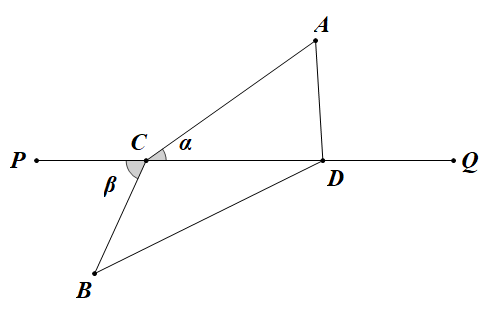
\includegraphics[width=0.4\textwidth]{1.png}
	\caption{}
\end{figure}\par
\textbf{解法1}({\fangsong 标准答案}):
\begin{figure}[htbp]
	\centering
	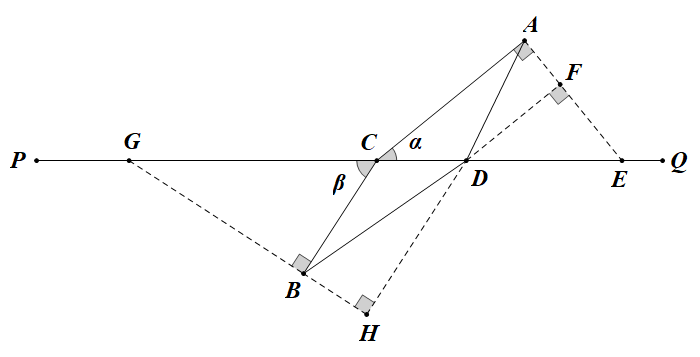
\includegraphics[width=0.6\textwidth]{2.png}
	\caption{}
\end{figure}
\par
如图2, 作$AE\perp AC$交$PQ$于$E$, 过$B$作$BG\perp BC$交$PQ$于$G$. 过$D$作$DF, DH\perp AE, BG$于$F, H$. 则$AD>FD$, $BD>HD.$\par
则有
\begin{align*}
	\frac{AC}{\cos{\alpha}}+\frac{BC}{\cos{\beta}}&=CE+GC=DE+DG=\frac{DF}{\cos{\alpha}}+\frac{DH}{\cos{\beta}}\\
	&<\frac{AD}{\cos{\alpha}}+\frac{BD}{\cos{\beta}}.
\end{align*}\\\par
\textbf{解法2}({\fangsong 程昊一}):\par
如图3, 过$D$作$DS, DT\perp AC, BC$于$S$, $T$. 则有$AD>AS$, $BD>BT$. 又因为$\alpha, \beta$均为锐角, 所以$\cos{\alpha}>0$, $\cos{\beta}>0$. 则
\begin{align*}
	\frac{AC-AD}{\cos{\alpha}}&<\frac{AC-AS}{\cos{\alpha}}=\frac{CS}{\cos{\alpha}}=CD=\frac{CT}{\cos{\angle TCD}}=\frac{BT-BC}{\cos{\beta}}\\
	&<\frac{BD-BC}{\cos{\beta}}.
\end{align*} 
即
\[\frac{AC}{\cos\alpha}-\frac{AD}{\cos\beta}<\frac{BD}{\cos\beta}-\frac{BC}{\cos\beta}.\]
移项, 即得结论.
\begin{figure}[htbp]
	\centering
	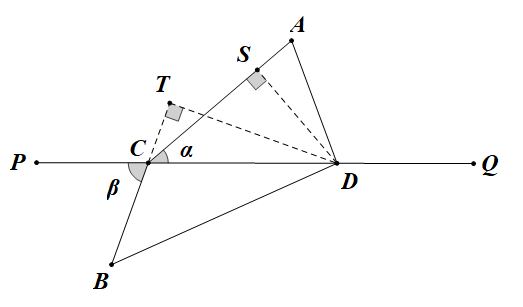
\includegraphics[width=0.5\textwidth]{3}
	\caption{}
\end{figure}\\\par
\textbf{解法3}({\fangsong 韦懿轩}):\par
如图4, 在射线$AC$, $BC$上截取$E$, $F$, 使得$AE=AD$, $BF=BD$. 过$E$, $F$作$EG, FH\perp AC, BC$于$G, H$. 连接$DE$, $DF$. 不妨设$D$在$C$左侧(另一种情况可以类似讨论).\par
因为
\[\angle CED=90^\circ+\frac{\angle A}{2}>90^\circ=\angle CEG,\]
所以$G$在$D$的左侧. 同理, $\angle BFD<\angle BFH$, 所以$H$在$D$的右侧. 那么有
\[CG<CH.\]\par
类似于解法2, 有
\[\frac{AC-AD}{\cos{\alpha}}=CG<CH<\frac{BD-BC}{\cos{\beta}}.\]
移项即得结论.
\begin{figure}[htbp]
	\centering
	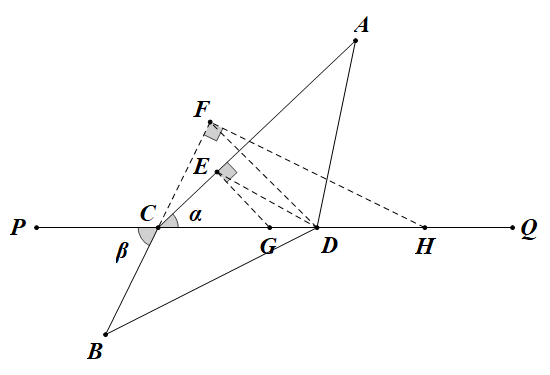
\includegraphics[width=0.4\textwidth]{4.png}
	\caption{}
\end{figure}\\\par 
\textbf{解法4}({\fangsong 马逸凡}):\par
如图5, 作点$F$, $H$使得$\angle ADF=\alpha$, $\angle BDH=\beta$, $\angle HBD=\angle FAD=90^\circ$. 过$F$, $H$作$FE, HG\perp PQ$于$E$, $G$. \par
则由$\angle DAF=\angle DEF$知$A$, $D$, $E$, $F$共圆. 则
\begin{align*}
	\angle DAE&=\angle DFR=90^\circ-\angle DFE=90^\circ-(\angle ADE-\angle ADF)\\
	&=90^\circ-(\angle ADE-\angle ACD)=90^\circ-\angle CAD.
\end{align*}
于是
\[\angle CAE=\angle CAD+\angle DAE=90^\circ.\]\par
同理, 有$\angle CBG=90^\circ$. 于是
\[\frac{AC}{\cos\alpha}=CE,\,\frac{AD}{\cos\alpha}=DF,\,\frac{BC}{\cos\beta}=CG,\,\frac{BD}{\cos\beta}=DH.\]
则
\[\frac{AD}{\cos\alpha}+\frac{BD}{\cos\beta}=DF+DH>DG+DE
=\frac{AC}{\cos{\alpha}}+\frac{BC}{\cos{\beta}}.\]

\begin{figure}[htbp]
	\centering
	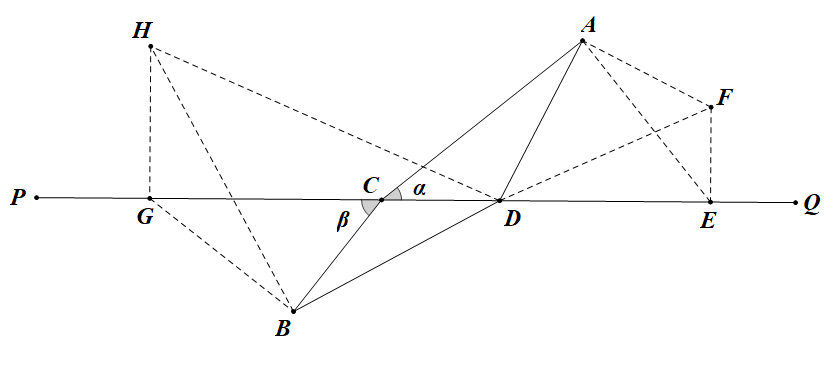
\includegraphics[width=0.6\textheight]{5.png}
	\caption{}
\end{figure}\par
\textbf{解法5}({\fangsong 李衡岳}):\par
如图6, 过$A$, $B$作$AS, BT\perp PQ$于$S, T$.\par 
以下只讨论$D$在线段$ST$内的情况. 这是因为, 若$D'$在线段$ST$外, 不妨设在射线$SQ$上. \par 
若$D'S\ge ST$, 则有$AC<AD'$, $BC<BD'$, 结合$\cos\alpha>0$, $\cos\beta>0$可知结论成立. 若$SD'<ST$, 则可在线段$ST$内取点$D$, 使得$DS=D'S$. 则此时$AD=AD'$, $BD'>BD$, 可化归为$D$在线段$ST$内. 因此, 只讨论$D$在线段$ST$内的情况.\par
设$SD=x$, $0\le x\le ST$. 则可知
\[\frac{AD}{\cos\alpha}+\frac{BD}{\cos\beta}=\frac{\sqrt{x^2+AS^2}}{\cos\alpha}+\frac{\sqrt{(ST-x)^2+BT^2}}{\cos\beta}.\]
记上式为$f(x)$. 通过并不困难的计算, 可以得到
\[f'(x)=\frac{-x}{\cos{\alpha}\sqrt{x^2+AS^2}}+\frac{ST-x}{\cos{\beta}\sqrt{(ST-x)^2+BT^2}}.\]\par
下面求$f(x)$的极值点. 令$f'(x)=0$, 移项并平方, 有
\[\frac{x^2}{\cos^2\alpha (x^2+AS^2)}=\frac{(ST-x)^2}{\cos^2\beta \left[(ST-x)^2+BT^2\right]}.\]
而\begin{align*}
	\frac{x^2}{\cos^2\alpha (x^2+AS^2)}&=\frac{\dfrac{1}{\cos^2\alpha}\left(\cos^2\alpha x^2+\cos^2\alpha AS^2\right)-AS^2}{\cos^2\alpha (x^2+AS^2)}\\
	&=\frac{1}{\cos^2\alpha}-\frac{AS^2}{\cos^2\alpha (x^2+AS^2)}.
\end{align*}
由于$0\le x\le ST$, 所以等式左边单调递增. 利用完全相同的方法可以说明, 等式右边单调递减. 则此方程有唯一的实根. 而将$x=SC$代入, 可以计算出等式左右两端相等, 即$x=SC$为方程的实根. \par
即, 方程有唯一的实根$x=SC$. 所以, $f(x)$有唯一的极值点$x=SC$. 而将$x=0$代入, 有
\[f(0)>f(SC),\]
即$x=SC$为$f(x)$的极小值点. 则, 对于任意的$x\neq CS$, $0\le x\le ST$, 有
\[f(CS)<f(x).\]\par
结合前面的讨论, 可知结论成立.

\begin{figure}[htbp]
	\centering
	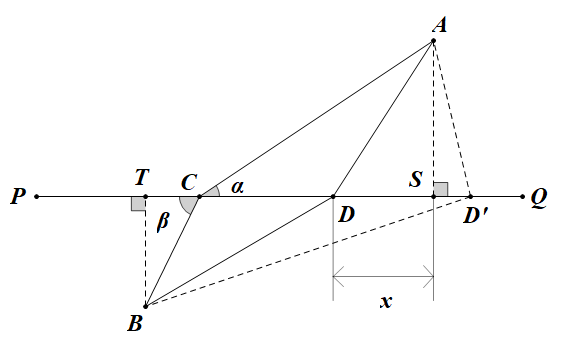
\includegraphics[width=0.5\textwidth]{6.png}
	\caption{}
\end{figure}\par
\textbf{解法6}({\fangsong 非严格}):\par
设想$PQ$两侧为不同的介质, 其光速分别为$c_1$与$c_2$. 光线从$A$出发, 经过$C$后折射到$B$, 如图7. 设入射角为$i$, 折射角为$\gamma$, 由光的折射定律, 有
\[\frac{c_1}{c_2}=\frac{\sin{i}}{\sin{\gamma}}=\frac{\cos{\alpha}}{\cos{\beta}}.\]
设
\[k=\frac{c_1}{\cos{\alpha}}=\frac{c_2}{\cos{\beta}}.\]\par
则
\[\frac{AC}{c_1}+\frac{CB}{c_2}=\frac{1}{k}\left(\frac{AC}{\cos\alpha}+\frac{CB}{\cos\beta}\right)\]
为光经过折线$ACB$所需时间. 同理,
\[\frac{1}{k}\left(\frac{AD}{\cos\alpha}+\frac{DB}{\cos\beta}\right)\]
为光从$A$到$D$, 再从$D$到$B$所需时间. 注意, 折线$ADB$并不是一条光路, 因为这违背了光的折射定律.\par
而根据费马原理, 光所经过的路线所花费的时间为稳定点\footnote{指一阶导数为$0$的点.}, 在这里是极小值. 所以, 光从$A$到$D$, 再从$D$到$B$所需时间一定大于光经过折线$ACB$所需时间. 因此
\[\frac{1}{k}\left(\frac{AC}{\cos\alpha}+\frac{CB}{\cos\beta}\right)<\frac{1}{k}\left(\frac{AD}{\cos\alpha}+\frac{DB}{\cos\beta}\right).\]
而$1/k>0$, 消去$1/k$即得结论.
\begin{figure}[htbp]
	\centering
	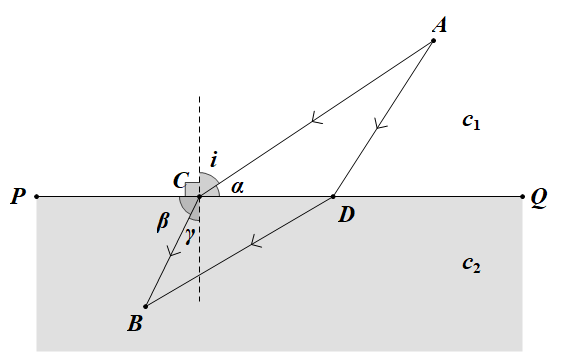
\includegraphics[width=0.45\textheight]{7.png}
	\caption{}
\end{figure}
\end{document}